%%%%%%%%%%%%%%%%%%%%%%%%%%%%%%%%%%%%%%%%%
% Laboratory Report LaTeX Template
%
% This template has been downloaded from:
% http://www.latextemplates.com
%
% Original header:
%
% This is a LaTeX version of the sample laboratory report
% from Virginia Tech's copyrighted 08-09 CHEM 1045/1046 lab manual.
% Reproduction of this one appendix section for academic purposes
% should fall under fair use.
%
%%%%%%%%%%%%%%%%%%%%%%%%%%%%%%%%%%%%%%%%%

%----------------------------------------------------------------------------------------
%	DOCUMENT CONFIGURATIONS
%----------------------------------------------------------------------------------------

\documentclass[a4paper,11pt,openbib]{report}
\usepackage[utf8]{inputenc} % Skal passe til editorens indstillinger
\usepackage[T1]{fontenc} % fonte (output)
\usepackage{lmodern} % vektor fonte
\usepackage{graphicx} % indsættelse af billeder
\graphicspath{{billeder/}} % stivej til bibliotek med figurer
\usepackage{mathtools} % matematik - understøtter muligheden for at bruge \eqref{}
\usepackage[draft,danish]{fixme}
\usepackage{sistyle}
\usepackage{blindtext}
\usepackage{tabularx}
\usepackage{pdflscape}
\usepackage[protrusion=true,expansion=true]{microtype}
\usepackage[hang,small,bf]{caption}
\usepackage{fancyvrb}
\usepackage{courier}
\usepackage[numbers]{natbib}
 \setcounter{secnumdepth}{3} % Paragraph bliver nummeret ligesom section
 \setcounter{tocdepth}{3}  % De bliver tilføjet til indeksering
% Indsæt todonotes i margin
\usepackage{todonotes}
\usepackage{pdfpages}
\SIdecimalsign{,}
\usepackage{textcomp}
\usepackage{listings}
\usepackage{color}
\usepackage{enumerate}
\usepackage{wrapfig}
\definecolor{listinggray}{gray}{0.9}
\definecolor{lbcolor}{rgb}{0.9,0.9,0.9}
\renewcommand\lstlistingname{Kodeeksempel}
\renewcommand\lstlistlistingname{Kodeeksempel}
%TEST
\newcommand\javakode{\renewcommand\lstlistingname{Kodeeksempel}}
\newcommand\pseudokode{\renewcommand\lstlistingname{Kodeeksempel}}
\newcommand\lstkode{\renewcommand\lstlistingname{Kodeeksempel}}

%CiteCMD
\def\citeAuthorNumber#1{[\citeauthor{#1}, \citep{#1}, \citeyear{#1}]}

% Custom commands
\newcommand{\sizeForIpadScreenShots}{0.2}
\newcommand{\newLine}{\newline\newline}


\lstset{
        basicstyle=\footnotesize\ttfamily, % Standardschrift
        numbers=left,               % Ort der Zeilennummern
        numberstyle=\color{blue!20!black!30!green}\tiny\ttfamily,          % Stil der Zeilennummern
        %stepnumber=2,               % Abstand zwischen den Zeilennummern
        numbersep=5pt,              % Abstand der Nummern zum Text
        tabsize=2,                  % Groesse von Tabs
        extendedchars=true,         %
        breaklines=true,            % Zeilen werden Umgebrochen
        keywordstyle=\color{red},
   		frame=b,         
%        keywordstyle=[1]\textbf,    % Stil der Keywords
%        keywordstyle=[2]\textbf,    %
%        keywordstyle=[3]\textbf,    %
%        keywordstyle=[4]\textbf,   \sqrt{\sqrt{}} %
        stringstyle=\color{blue}\ttfamily, % Farbe der String
        showspaces=false,           % Leerzeichen anzeigen ?
        showtabs=false,             % Tabs anzeigen ?
        xleftmargin=17pt,
        framexleftmargin=17pt,
        framexrightmargin=5pt,
        framexbottommargin=4pt,
        %backgroundcolor=\color{lightgray},
        showstringspaces=false,      % Leerzeichen in Strings anzeigen ?  
		inputencoding=utf8,
		  literate={å}{{\aa}}1
		                {æ}{{\ae}}1
		                 {ø}{{\o}}1      
}

\lstloadlanguages{% Check Dokumentation for further languages ...
        %[Visual]Basic
        %Pascal
        C,
        %C++
        %XML
        %HTML
        Java
}
\DeclareCaptionFont{white}{\color{white}}
\DeclareCaptionFormat{listing}{\colorbox[cmyk]{0.43, 0.35, 0.35,0.01}{\parbox{\textwidth}{\hspace{15pt}#1#2#3}}}
\captionsetup[lstlisting]{format=listing,labelfont=white,textfont=white, singlelinecheck=false, margin=0pt, font={bf,footnotesize}}

\usepackage{subfigure}
\usepackage{subfloat}
%\usepackage{geometry}
%\geometry{left=3.3cm,top=3cm,right=2.8cm,bottom=3.5cm}
\usepackage{booktabs,dcolumn,array}
\usepackage{multirow}
\renewcommand\multirowsetup{\centering}
\usepackage{cellspace}
	\addtolength\cellspacetoplimit{4pt}
	\addtolength\cellspacebottomlimit{4pt}
%\renewcommand\baselinestretch{1.6}

%\settocdepth{subsection}
%\setsecnumdepth{subsection}

\usepackage[plainpages=false,pdfpagelabels,pageanchor=false]{hyperref} % aktive links
%\hypersetup{%
\usepackage{memhfixc}% rettelser til hyperref

% -- Vis equations og figurere med chapter nummer først for bedre overskuelighed.
\numberwithin{equation}{chapter}
\numberwithin{figure}{chapter}

\usepackage{fancyhdr}


%Opsætning af marginer
\addtolength{\hoffset}{-0.3cm}
\addtolength{\textwidth}{2cm}
\addtolength{\voffset}{-1.8cm}
\addtolength{\textheight}{4.8cm}
\topmargin = 0cm
\setlength{\parindent}{0pt} % Sørger for at der ikke sker nogen indrykning ved nyt afsnit.

\pagestyle{fancyplain}

%Opsætninger af Header og Footer
\renewcommand{\chaptermark}[1]{\markboth{\thechapter.\ #1}{}}
\fancyhf{}
\lhead{\bfseries \leftmark}
\rhead{\bfseries \thepage}
\renewcommand{\headrulewidth}{0.5pt}
\renewcommand{\footrulewidth}{0.5pt}
\renewcommand{\headwidth}{15.9cm}
\addtolength{\headheight}{0.5pt}

\fancypagestyle{plain}{\renewcommand{\headrulewidth}{0.5pt}}
% Alle forsider er plain, og kan sættes op her.
\fancypagestyle{empty}{\renewcommand{\headrulewidth}{0pt} \renewcommand{\footrulewidth}{0pt} \lhead{} \rhead{}}

\fancypagestyle{lines}{\renewcommand{\headrulewidth}{0.5pt} \lhead{} \rhead{}}
% Siderne med Forord og Indholdsfortegnelse skal ikke have titel og nummerering, dette er opsat her.


%OpsÔøΩtning af Chapters
\makeatletter
\def\thickhrulefill{\leavevmode \leaders \hrule height 1ex \hfill \kern \z@}
\def\@makechapterhead#1{\vspace*{-10\p@}{\parindent \z@ {\raggedright \LARGE \bfseries \thechapter \;} \LARGE \bfseries #1}\vskip 10 \p@}
\def\@makeschapterhead#1{\vspace*{-10\p@}{\parindent \z@ {\raggedright \Huge \bfseries #1}\vskip 10 \p@}}

\setlength{\headheight}{14pt}

\usepackage[numbib,nottoc]{tocbibind}


%\title{LAB-1 for EMB-1} % Title

%\author{author} % Author name

\begin{document}
\thispagestyle{empty}

\begin{minipage}{\textwidth}
\flushright

% ----------------------------------------------------------------------------------
% ---- Titel på Rapport
% ----------------------------------------------------------------------------------
\begin{flushright}
{\huge\bfseries Project plan}
\end{flushright}
% ----------------------------------------------------------------------------------

\noindent\rule[-1ex]{\textwidth}{2pt}\\
[2.5ex]
% ----------------------------------------------------------------------------------
% ---- Underoverskrift på rapport
% ----------------------------------------------------------------------------------
\hfill\emph{\Large Robotic system design}
% ----------------------------------------------------------------------------------
\end{minipage}
\\
\\
\\
\\
\begin{figure}[ht]
\centering
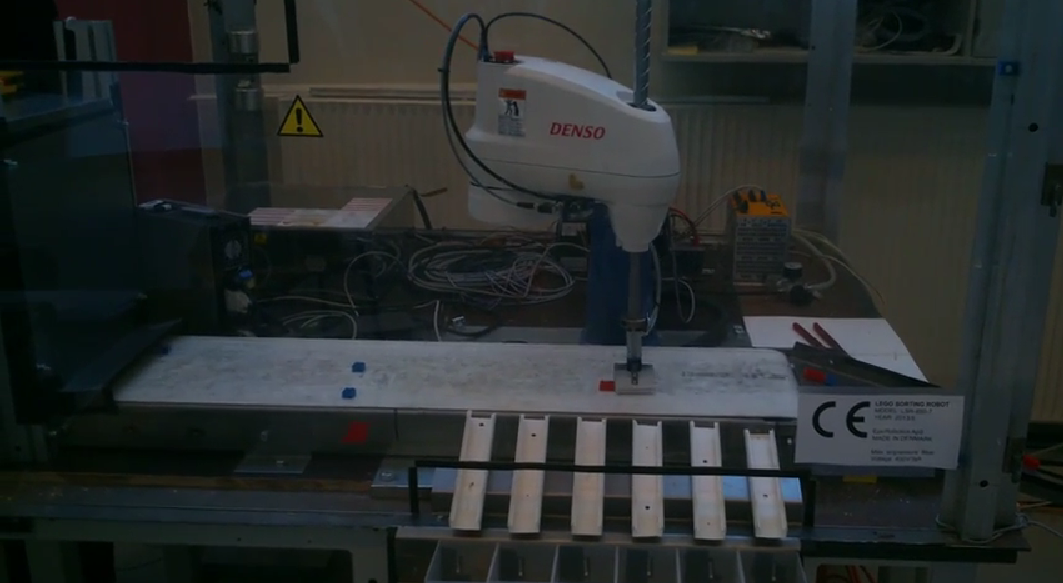
\includegraphics[width=\textwidth]{images/frontpage.png}
\label{fig:frontpage}
\end{figure}
\@afterindentfalse \@afterheading

\vspace{2cm}
\begin{minipage}{\textwidth}
\flushleft


\end{minipage}

\vspace{\stretch{1}}
\begin{minipage}{\textwidth}
\flushright

%----------------------------------------------------------------------------------
% ---- NAVN
%----------------------------------------------------------------------------------
{\bfseries Group 3:\\}
Anders Prier Lindvig \\
Lasse Engberg Andersen  \\
Michael Lau Sørensen \\
Stoyan Stoyanov \\
Christian Liin Hansen \\ 
[1ex]

%----------------------------------------------------------------------------------
% ---- NAVN På VEJLEDER
%----------------------------------------------------------------------------------
 {\bfseries Instructors:\\}
Jens Cortsen \\
Kjeld Jensen \\
Ole Dolriis \\
[1ex]

%----------------------------------------------------------------------------------
% ---- NAVN På Projectejer
%----------------------------------------------------------------------------------
% {\bfseries Project owner:\\}
%ImproSeed ApS\\ 
%[1ex]

%----------------------------------------------------------------------------------
% ---- UNDERVISNINGSSTED
%----------------------------------------------------------------------------------
{\bfseries University:\\}
The Technical Faculty, University of Southern Denmark\\
[1ex]
%----------------------------------------------------------------------------------


%----------------------------------------------------------------------------------
% ---- KURSUS
%----------------------------------------------------------------------------------
{\bfseries Course:\\}
RMRSD1. 10 ECTS point\\
[1ex]

%----------------------------------------------------------------------------------
% ---- PERIODE
%----------------------------------------------------------------------------------
{\bfseries Project period:\\}
September 1$^{st}$ 2014 - January 1$^{st}$ 2015 \\

\end{minipage}

\setlength\parindent{0pt} % Removes all indentation from paragraphs

\renewcommand{\labelenumi}{\alph{enumi}.} % Make numbering in the enumerate environment by letter rather than number (e.g. section 6)
\newpage
\tableofcontents
\newpage

\chapter{Introduction}
Robotic system design is a mandatory course on the 3rd semester in the robotic systems master program. The course contains 6 student groups, where each has been selected to work with either a mobile robot or workcell robot. This group 3 is working with the workcell robot, i.e PA10 or Staubli robot. The project goals is to create a solution among all the groups to manufacture a multi robot production facility that handles LEGO-bricks orders. The worokcell robots will sort the LEGO-bricks and the mobile robots will handle transportation. A LEGO-dispenser will be available in the project, which will provide the system with LEGO-bricks. The scene will take place in the RoboLab at the university. 
\\
\\
The scene in Robolab has been illustrated, with reference to the course description, in figure \ref{fig:workZone}. Here there will be 3 mobile robots and 3 workcell robots working together to perform the project goal. 


\begin{figure}[ht]
\centering
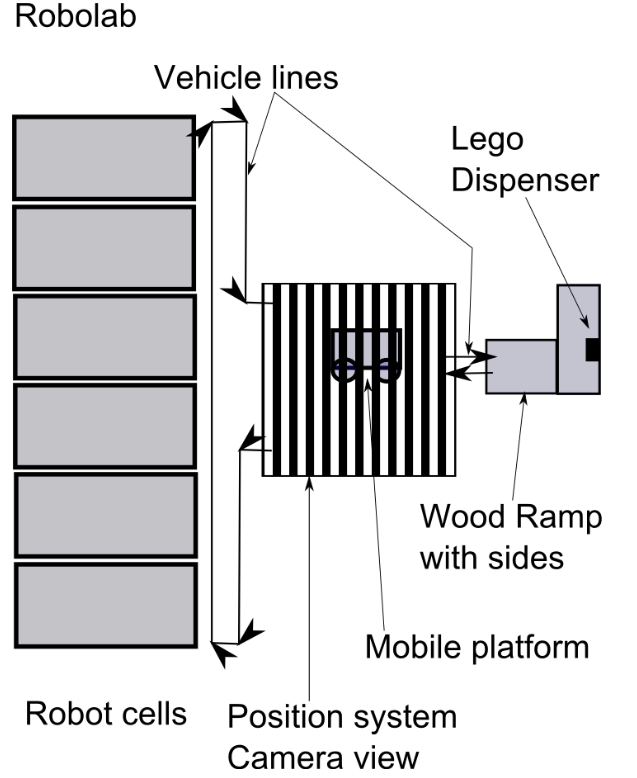
\includegraphics[scale=0.4]{images/workZone.png}
\caption{Setup of the multi robot production facility, where workcell robots sorting LEGO bricks in robot cells and mobile robots transport the LEGO-brick in Robolab}
\label{fig:workZone}
\end{figure}

\section{Project setup}
A general block diagram was created to start identifying different components for the system in the robot cell. This is illustrated in figure \ref{fig:hardwarediagram}. 

In overall the system for the robot cell contains the following components
\begin{itemize}
\item{PA10 or Staubli workcell robot}
\item{Conveyor belt}
\item{Carmine RGB-D sensor}
\item{PLC}
\item{Motor controller for the conveyor belt}
\item{Protocol interface to MES server}
\end{itemize}

\begin{figure}[ht]
\centering
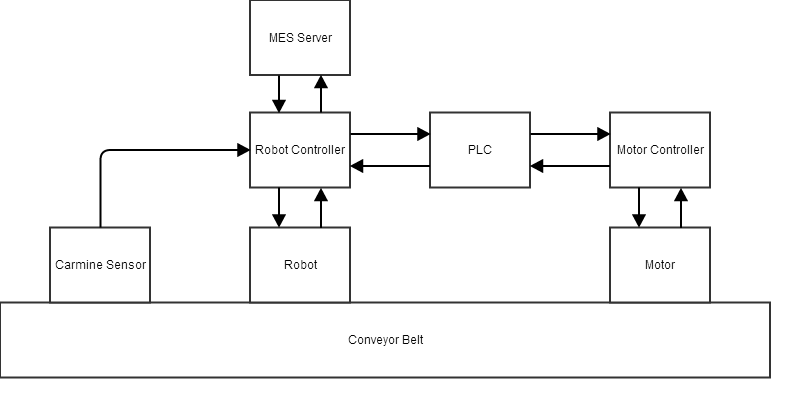
\includegraphics[width=\textwidth]{images/hardwarediagram.png}
\caption{Generel blockdiagram of the different component for the system of the workcell robot in the robot cell}
\label{fig:hardwarediagram}
\end{figure}

%\section{Project description}
%Initially the workcell robot is standing in a initial configuration and the system in the robot cell is waiting for status request or order request from the MES server. If an order is placed in the MES system, an mobile robot will be ordered to pick up bricks from the LEGO dispenser, which feed the mobile robot with a random number of LEGO bricks in a random shape and color. However limitations on the LEGO-bricks will be stated later in the project. 
%
%The MES server will be sending status request for all the robot workcell and receive status if workcells are available or not.
%While the mobile robot has been received LEGO-bricks from the dispenser, the MES server has arranged which workcell the current mobile robot has to go to. After the mobile robot acknowledge this order, MES server is sending status report to system in workcell. While mobile robot is under way, the system in workcell gets ready for incomming load-off. The moment the mobile robot get to the barcode, that indicate the target workcell, the mobile robot will send status to the MES server. The MES server will then send loading request to the given workcell, in order begin the loading and sorting of LEGO-bricks.  The workcell system will send status report back to MES server to indicate that the system is in process of sorting. The MES sever are able to send the mobile robot back to initial waiting position in the local GPS zone. Doing the sorting procedure, all the LEGO bricks will be places in either a order box or spare-part box. When the system in the workcell is done sorting LEGO bricks, the status of boxes is send back to the MES server. If the order is not finish, collecting LEGO bricks procedure will be executed. If the order is finish, collecting orders procedure will be executed, i.e mobile robot will be ordered to go to the current workcell and pick up the order box. If the spare-part box are reaching its maximum capacity, the MES server will be informed, which creates an order procedure. 

\chapter{Diagrams}
In this chapter, the loading procedure and unloading procedure will be explain. The loading procedure is related to the workcell, which means that LEGO bricks are moved from the mobile robot to the workcell. The unloading procedure is the opposite, i.e. LEGO bricks are moved from the workcell to the mobile robots.

\section{Loading LEGO bricks to workcell procedure}
The workcell will receive an order message from the MES server. It will activate the conveyer belt and then wait for a lego brick to be detected, by the vision system. If the vision system detects a LEGO brick the workcell robot will move to the LEGO brick and grasp it. The information used for the grasping is position, orientation and velocity acquired from the vision system and the vision velocity feedback respectively. The workcell robot then moves to either the order box or the leftover box, depending upon the LEGO brick. It will then ungrasp the LEGO brick. This will continue until the order is complete. A message will then inform the MES server that the order has been fulfilled. A block diagram of this process can be observed in figure \ref{fig:overall_block_diagram_loading}.

\begin{figure}[ht]
\centering
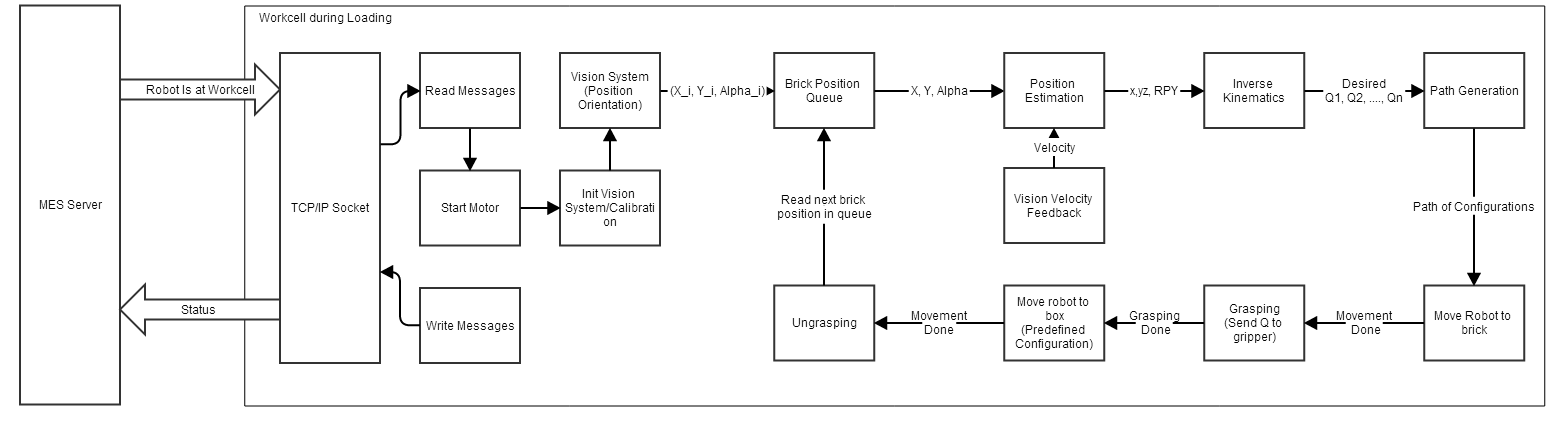
\includegraphics[width=\textwidth]{images/overall_block_diagram_loading.png}
\caption{Diagram illustration the loading procedure}
\label{fig:overall_block_diagram_loading}
\end{figure}


\section{Unloading LEGO bricks to mobile robot procedure}
When the workcell robot has finished sorting the LEGO bricks, a message to the MES will be sent. When a mobile robot has arrived at the end of the conveyor belt the workcell robot will then move to a predefined position for grasping the boxes of lego bricks. While holding the LEGO box the workcell robot now moves the box to the conveyor belt and places it in a predefined position on the belt. The conveyor belt then moves the box to the waiting mobile robot and after a certain amount of time, the belt is stopped. It will then be considered if new boxes are need for further work. The workcell robot then returns to its loading state and send a message to the MES server indicating it is ready for a new order. A block diagram of this process can be observed in figure \ref{fig:overall_block_diagram_unloading}.

\begin{figure}[ht]
\centering
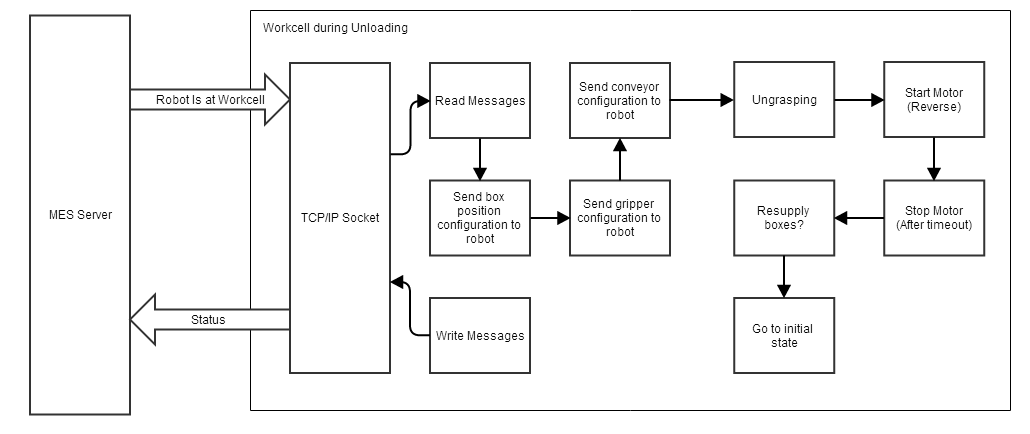
\includegraphics[width=\textwidth]{images/overall_block_diagram_unloading.png}
\caption{Diagram illustration the unloading procedure}
\label{fig:overall_block_diagram_unloading}
\end{figure}

\chapter{Tasks to be done}
Software tools installation:

\begin{itemize}
\item{ROS}
\item{RobWork}
\item{OpenCV}
\item{MES}
\end{itemize}

The first steps after the initial project design are to install the required software tools. The system will mainly be running in ROS but it will also use different tools integrated with it for the different tasks. The kinematics/planning/grasping tasks will be implemented in RobWork which will be communicating to ROS. The vision part will be implemented with OpenCV which will have interface to ROS. The project managing system will be implemented as a MES Server in ROS and it will be communicating with a custom protocol, which will be implemented later on, with all the other branches of the system. After the required software tools are installed the next step will be to interface the group computers to the master computer in the work cell. As a beginning a communication within ROS should be established, meaning that the group members should be able to read from and write to ROS topics on the master computer. Afterwards, all the software tools should be interfaced to ROS.

\begin{itemize}
\item{PLC conveyor control}
\item{Template ROS nodes}
\item{Grasping Simulation}
\item{Color masks}
\item{Speed calculation}
\end{itemize}

There are several goals that have to be accomplished for the midterm demonstration. As a start the PLC should be interfaced to ROS and be able to control the conveyor belt at least in one direction with fixed speed. Several “template” ROS nodes have to be created that are able to communicate with each other. Regarding the kinematics/grasping/planning task a simulation of a grasping of an object have to be implemented in RobWork. For the vision part several masks should be created that are able to distinguish bricks with different colors. Finally it is desirable speed calculation to be implemented within the vision system.


\chapter{Ideas for final implementation}
Different solution for having a multi robot production facility has been discussed among the group. These discussion will be discussed among the other groups in the RSD course. A data flow diagram is shown in figure \ref{fig:ideasForImplementation}. 

\begin{figure}[ht]
\centering
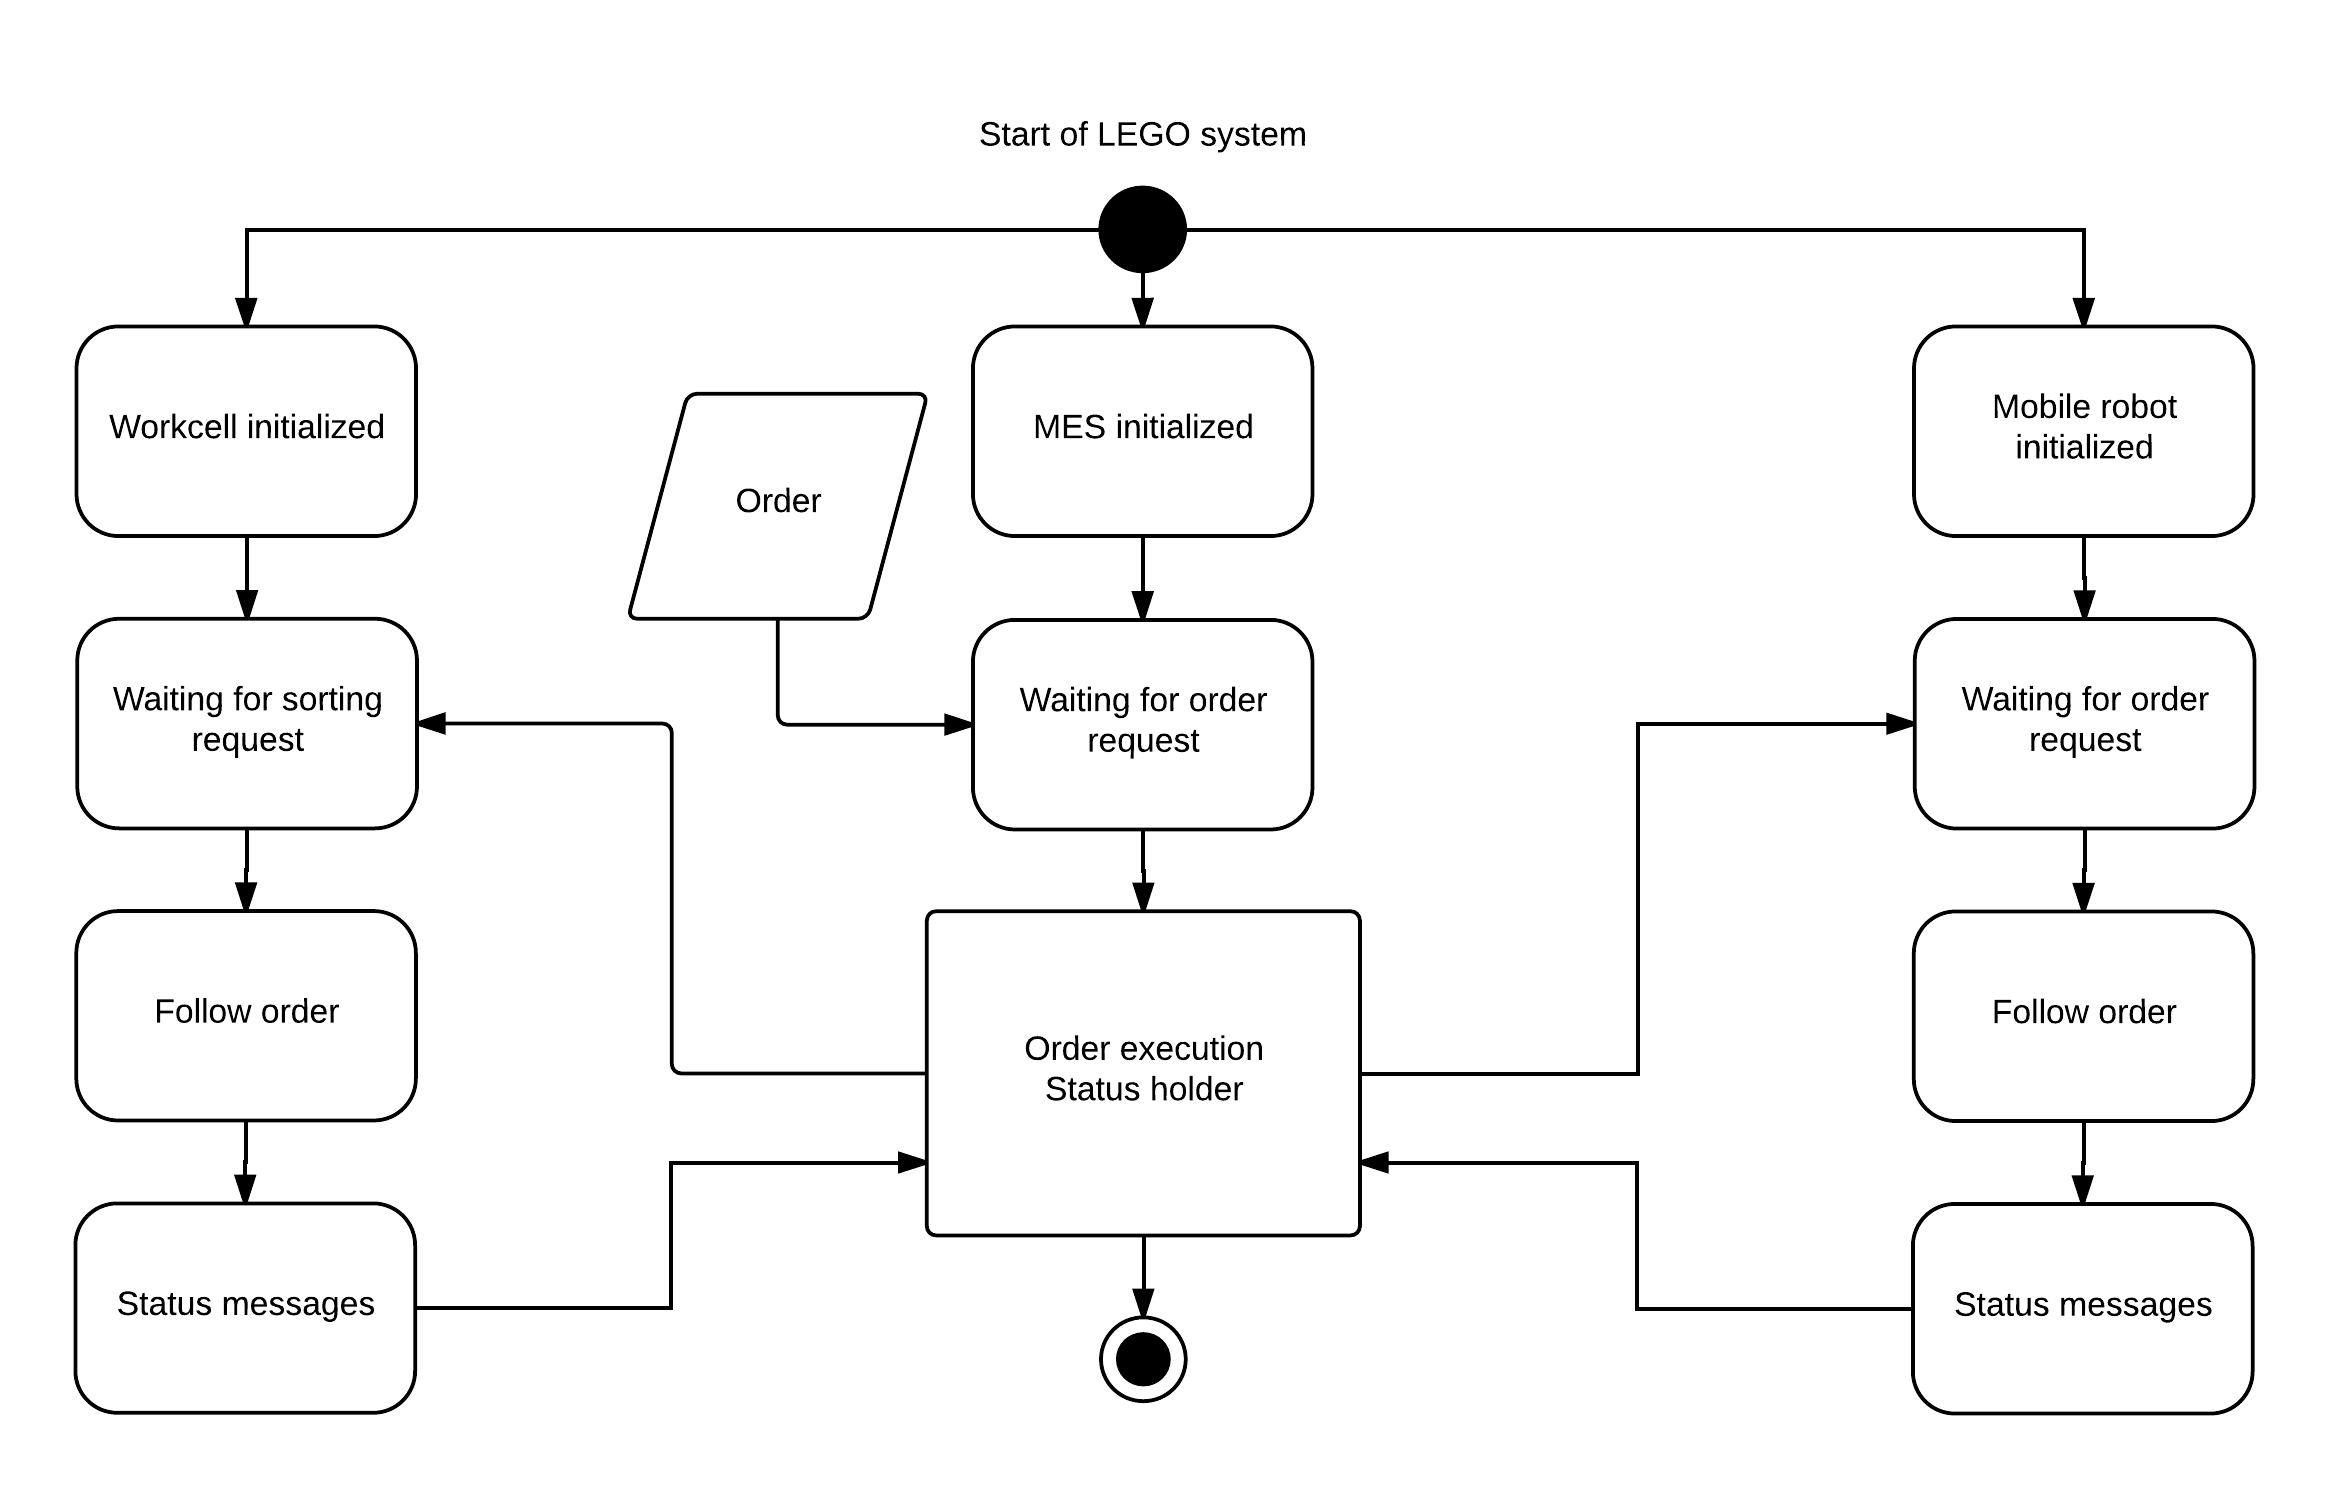
\includegraphics[width=\textwidth]{images/ideasForImplementation.png}
\caption{Idea for flow diagram between MES server, mobile robot and workcell robot}
\label{fig:ideasForImplementation}
\end{figure}

Initially the workcell robot is standing in a initial configuration and the system in the robot cell is waiting for status request or order request from the MES server. If an order is placed in the MES system, an mobile robot will be ordered to pick up bricks from the LEGO dispenser, which feed the mobile robot with a random number of LEGO bricks in a random shape and color. However limitations on the LEGO-bricks will be stated later in the project. 

The MES server will be sending status request for all the robot workcell and receive status if workcells are available or not.
While the mobile robot has been received LEGO-bricks from the dispenser, the MES server has arranged which workcell the current mobile robot has to go to. After the mobile robot acknowledge this order, MES server is sending status report to system in workcell. While mobile robot is under way, the system in workcell gets ready for incomming load-off. The moment the mobile robot get to the barcode, that indicate the target workcell, the mobile robot will send status to the MES server. The MES server will then send loading request to the given workcell, in order begin the loading and sorting of LEGO-bricks.  The workcell system will send status report back to MES server to indicate that the system is in process of sorting. The MES sever are able to send the mobile robot back to initial waiting position in the local GPS zone. Doing the sorting procedure, all the LEGO bricks will be places in either a order box or spare-part box. When the system in the workcell is done sorting LEGO bricks, the status of boxes is send back to the MES server. If the order is not finish, collecting LEGO bricks procedure will be executed. If the order is finish, collecting orders procedure will be executed, i.e mobile robot will be ordered to go to the current workcell and pick up the order box. If the spare-part box are reaching its maximum capacity, the MES server will be informed, which creates an order procedure. 

\section{Camera mounting}
The camera needs to cover a field of view, that contains an sufficient area of the conveyor belt. Having the camera mounted with the optical axis perpendicular to the plane of the conveyor belt is optimal. However the camera needs to be mounted with a given clearance to avoid collision with the work cell robot. An idea is to mount a steal frame around the conveyor belt and having the camera mounted on the frame. Thereby it is possible to have a fixed mounted camera  on top of the conveyor belt and protected from colliding with the workcell robot. An illustration of the idea is shown in figure \ref:

%\listoftodos

%----------------------------------------------------------------------------------------
%	BIBLIOGRAPHY
%----------------------------------------------------------------------------------------
\pagebreak % Bibliografier
\include{biblio/bib}

\end{document}